\documentclass{beamer}

\usepackage[utf8]{inputenc} %cp1252 pour Windows, utf8 pour Linux
\usepackage[T1]{fontenc}
\usepackage{lmodern}
\usepackage{graphicx}
\usepackage[frenchb]{babel}
\usepackage{hyperref}

\usetheme{Warsaw}

\setbeamertemplate{blocks}[rounded]%
[shadow=true]

\title{La guerre numérique, une réalité !}

\author{Corentin \bsc{CHÉDOTAL}}


\date{30 Mars 2016}

\subject{Cyberguerre}

\AtBeginSubsection[]
{
  \begin{frame}<beamer>{Sommaire}
    \tableofcontents[currentsection,currentsubsection]
  \end{frame}
}

\begin{document}

\begin{frame}
  \titlepage
\end{frame}

\begin{frame}{Sommaire}
  \tableofcontents
\end{frame}

\begin{frame}{Préface}
    \begin{alertblock}{Nota}
        La cyberguerre et ce qui l'entoure est fréquemment affiliée au monde des renseignements. Ainsi les informations sur celle-ci sont généralement entourées du film opaque de la classification des documents. De ce fait certains des éléments contenus dans cette présentation se révéleront peut être incomplets ou inexacts dans le futur suite à des déclassifications.
    \end{alertblock}
\end{frame}

\section{Introduction}

\begin{frame}{Ouverture}
  \begin{quotation}
    [Le Cyber], est un milieu à part entière, d'une complexité extrême. Et qui voit actuellement des combats d'une ampleur, je serais même tenté de dire d'une violence, inouïe.\\
    Matrix n'est plus un film de science-fiction, nous y sommes.
  \end{quotation}
  Jean-Yves \bsc{Le Drian}, Ministre de la Défense\\
  Janvier 2016
\end{frame}

\begin{frame}{La guerre du numérique, késako ?}

    Internet connecte presque tous les réseaux. Ainsi l'information peut être transmise d'un bout à l'autre de n'importe quel endroit sur Terre à n'importe quel autre. Les états comme les entreprises et les particuliers se servent donc d'Internet continuellement.\\ Cependant aucun réseau n'est infaillible.\\
    Les informations ont de la valeur.\\
    De plus en plus de systèmes sont connectés à Internet, de la webcam de votre maison à des fonderies.\\
    Alors des acteurs rivaux tenteront toujours d'employer tous les moyens à leur disposition pour contrer leurs nemesis.

\end{frame}

\begin{frame}{Divers termes pour décrire une même réalité}
    
Partant du constat précédent le cyberespace est bien un champ de bataille.\\
\vspace{10pt}
L'OTAN préfèrera employer le terme de "cyberdéfense" et évitera à tout prix celui de "cyberguerre" qu'elle estime ne pas encore être une réalité pour diverses raisons.\\
\vspace{10pt}
La France depuis plusieurs années communique sur ce qu'elle qualifie de "4ème milieu" sur lequel se déroule des batailles aux effets parfois très réels. Le terme de "cyberguerre" étant alors employé parfois pour décrire ces conflits virtuels.

\end{frame}

\begin{frame}{Petit point de vocabulaire}
    
    \uncover<2->{%
    \begin{alertblock}{Cyberespace}
        Monde virtuel dans lequel l'Utilisateur se plonge quand il rentre dans un réseau.
    \end{alertblock}
    }

    \uncover<3->{%
    \begin{alertblock}{Sécurité des Systèmes d'Information}
        Ensemble des systèmes assurant à un SI\\
        \begin{itemize}
            \item sa confidentialité
            \item son intégrité
            \item sa disponiblité
            \item sa non-répudiation (authentification)
        \end{itemize}
    \end{alertblock}
    }
    
\end{frame}

\begin{frame}{Petit point de vocabulaire}{Les faux semblants}
    
    \uncover<2->{%
    \begin{alertblock}{Cyberprotection}
        Ensemble des moyens mis en place pour la protection des SI par un pays.
    \end{alertblock}
    }
    
    \uncover<3->{%
    \begin{alertblock}{Cyberdéfense}
        Défense et attaque de SI et/ou de réseaux par un pays.\\
        Décrit aussi la mise en place des stratégies et tactiques liées à ces attaques sans qu'elles ne soient forcément mise en oeuvre effectivement.
    \end{alertblock}
    }
    
    \uncover<4->{%
    \begin{alertblock}{Cyberrésilience}
        Autonomie des SI et réseaux par rapports à des états/entreprises ou à la nature.
    \end{alertblock}
    }
    
\end{frame}

\begin{frame}{Petit point de vocabulaire}{Les faux semblants}

    \uncover<2->{%
    \begin{alertblock}{Cybersécurité}
        Cyberprotection + Cyberdéfense + Cyberrésilience
    \end{alertblock}
    }

\end{frame}

\section{Les Acteurs}

\subsection{États}

\begin{frame}{"Five Eyes"}{Qu'est-ce ?}

    \begin{figure}[h]
        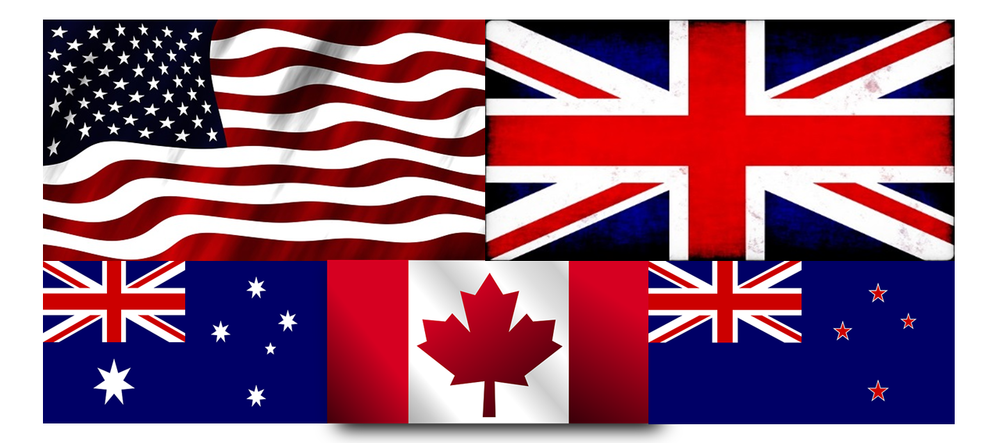
\includegraphics[scale=0.1]{FiveEyesFlags}
    \end{figure} 

Le "Five Eyes" est une alliance stratégique regroupant l'Australie, le Canada, la Nouvelle-Zélande, le Royaume-Uni et les États-Unis d'Amérique. Les agences de renseignements des cinq états membres sont en lien direct et doivent partager leurs renseignements bruts avec leurs homologues étrangers.\\
\vspace{10pt}
Dans le domaine du cyber cette alliance fait majoritairement dans la collecte passive de renseignement et dans la défense des infrastructures connectées à Internet de leurs pays respectifs.\\ 
Mais pas que\dots

\end{frame}

\begin{frame}{"Five Eyes"}{Pas très offensif ? Vraiment ?}
    
    \begin{figure}[h]
        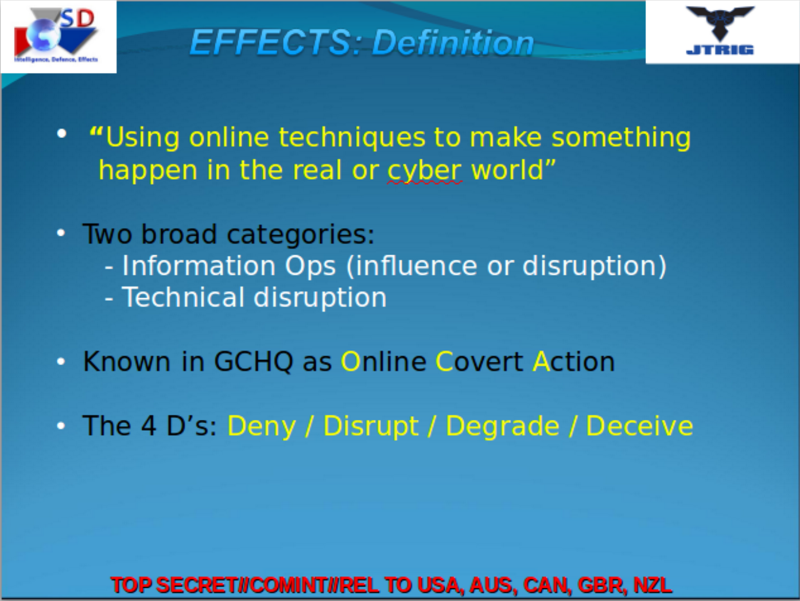
\includegraphics[scale=0.25]{SlideOCA}
        \caption{\label{SlideOCA} Extrait d'une présentation interne des services secrets britanniques} 
    \end{figure} 

\end{frame}

\begin{frame}{"Five Eyes"}{Le cas particulier des États-Unis d'Amérique}

En plus de leur participation au "Five Eyes" les États-Unis sont un cas particulier.\\
Bien plus agressifs que le reste des pays participants ils organisent leur collecte de renseignements de façon bien plus offensive, cassant les réseaux internes de certaines ambassades par exemple.\\
\vspace{10pt}
De plus les Américains ne s'arrêtent pas simplement à la défense et aux renseignements. Ils seraient à l'origine de plusieurs malwares dont le but était bien stratégique, dont \emph{Stuxnet}.

\end{frame}

\begin{frame}{L'État d'Israël}

    \begin{figure}[h]
        
\includegraphics[scale=0.2]{Flag_of_Israel}
    \end{figure}
    
    Au vu de l'histoire courte mais pourtant très belliqueuse d'Israël cela ne surprend personne de voir à quelle vitesse ce pays a pu utiliser l'informatique pas seulement pour la collecte d'information mais bien en tant qu'arme. Cependant très peu d'informations fuient dans le public sur leurs avancées.
    
    \uncover<2->{%
    \begin{block}{Stuxnet}
        Ver informatique découvert en 2010.
        Spécifique à Windows, il s'est propagé sur Internet jusqu'à atteindre sa seule et unique cible : le programme nucléaire iranien.
        Il a provoqué la destruction de centrifugeuse d'enrichissement d'uranium et plusieurs explosions.
        Enfin il avait un mécanisme d'auto-destruction.
    \end{block}
    }

\end{frame}

\begin{frame}{La Fédération de Russie}

    \begin{figure}[h]
        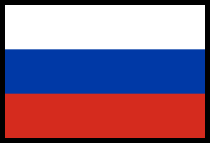
\includegraphics[scale=0.2]{Flag_of_Russia}
    \end{figure}
    
    La Russie est un des plus gros acteurs de la cyberguerre mais aussi l'un des mieux préparé à celle-ci. En effet, quand beaucoup d'états se satisfaissent simplement d'une cyberdéfense la Russie cherche elle une capacité offensive dans le Cyber et l'a, ce qui est en totale adéquation avec ses objectifs géopolitiques. De plus la Russie met un point d'honneur à rendre les liens entre les attaques et sont gouvernement extrêmement ténus. En effet elle emploiera des groupes et/ou des entreprises privés qui eux seront à l'origine des attaques.

\end{frame}

\begin{frame}{La Fédération de Russie}{Quelques exemples}

    \uncover<2->{%
    \begin{block}{Attaques sur les pays baltes}
        En 2008 l'Estonie puis la Lituanie subissent une vague d'attaques informatiques. Du simple \emph{defacing} à des tentatives d'accès à la banque centrale lituanienne. Les enquêtes pointent du doigt la provenance russe des attaques. Cependant elles proviennent de très nombreux particuliers et petits groupes, pas d'institutions gouvernementales. Aucune réelle sanction ne pourront être imposé par les états cibles.
    \end{block}
    }

    \uncover<3->{%
    \begin{block}{BlackEnergy}
        Trojan découvert d'abord en 2014, il est passé de la collecte de renseignements sur le gouvernement Ukrainien à la coupure temporaire récente du réseau électrique du pays.
    \end{block}
    }
    
\end{frame}

\begin{frame}{La République Populaire Démocratique de Corée}

    \begin{figure}[h]
        
\includegraphics[scale=0.2]{Flag_of_North_Korea}
    \end{figure} 

La Corée du Nord fait des efforts considérables depuis l'avènement des années 2000 pour maintenir une force offensive dans le Cyber. En effet, n'ayant que peu de capacités militaires conventionnelles elle se tourne vers d'autres moyens d'atteindre ses cibles principales : la République de Corée, le Japon et les États-Unis. Pour cela elle possède diverses institutions spécialisées dans le vol de renseignements et l'attaque de SI.

    \uncover<2->{%
    \begin{block}{Bureau 121 et The Interview}
        L'une des actions nord-coréennes les plus médiatisées fut l'attaque des serveurs de Sony Pictures qui annula la diffusion du film en salle comme l'attaque était accompagnée de menaces.
    \end{block}
    }

\end{frame}

\begin{frame}{La République Française}

    \begin{figure}[h]
        
\includegraphics[scale=0.2]{Flag_of_France}
    \end{figure} 

La France comme beaucoup d'états démocratiques et se disant des Droits de l'Homme tend à limiter son action à la cyberprotection et à l'aspect plus défensif de la cyberdéfense. Cependant il n'est pas exclus que la France prépare ou ait préparé des capacités offensives à employer si un conflit ouvert avait lieu avec une autre puissance mondiale. De plus la Loi sur le Renseignement récemment promulguée ouvre un plus grand panel de possibilité pour la DGSE.\\
Quant aux renseignements la France n'est pas en reste et utilise tous ses moyens à disposition pour faire de la collecte, y compris dans le cyberespace. 

\end{frame}

\begin{frame}{La République Française}{Quand la France embête ses alliés}
    
    \begin{figure}[h]
        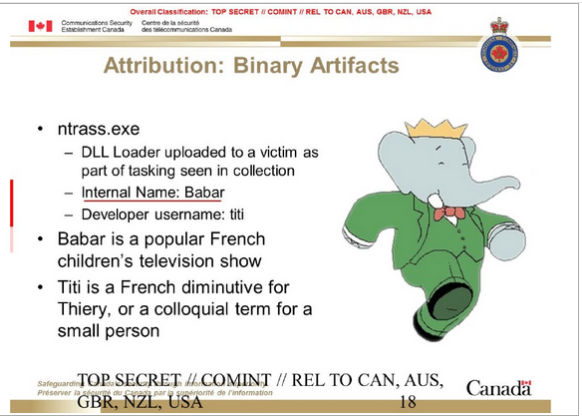
\includegraphics[scale=0.35]{BabarVirus}
        \caption{\label{SlideBabar} Rapport des services secrets canadiens sur Babar} 
    \end{figure}

\end{frame}

\subsection{Non-étatiques}

\begin{frame}{Anonymous}

    \begin{figure}[h]
        
\includegraphics[scale=0.15]{Anonymous_emblem}
    \end{figure}

Collectif anarchique d'\emph{hacktivistes} qui malgré son fonctionnement volontairement sans réelles règles parvient à réaliser de nombreuses actions de très grandes envergures.\\ Utilise l'informatique pour lutter contre le non respect de droits qu'ils considèrent fondamentaux. Leurs cibles les plus connues sont les gouvernements occidentaux, Daesh et la Scientologie.

    \uncover<2->{%
    \begin{block}{Actions couramment entreprises}
        \begin{itemize}
            \item Attaques DDoS
            \item \emph{Doxxing} de personnalités importantes de leurs cibles
            \item \emph{Defacing} des sites Internet de leurs cibles diverses
        \end{itemize}
    \end{block}
    }

\end{frame}

\begin{frame}{Daesh}

Organisation terroriste basée entre la Syrie et l'Irak, tristement célèbre en particulier suite aux attentats de Paris et de Bruxelles. Elle aurait une ou plusieurs "sections" dédiées à ce qu'elle qualifie de "cyberjihad". Cependant contrairement au reste de l'organisation leur "cyberjihad" est assez risible.

    \uncover<2->{%
    \begin{block}{Actions couramment entreprises}
        \begin{itemize}
            \item \emph{Defacing} de divers sites Internet
            \item Serait en train d'entreprendre des hacks bien plus importants
        \end{itemize}
    \end{block}
    }


\end{frame}

\begin{frame}{4chan}

Forum de discussion anglophone basé sur l'anonymat, il est extrêmement controversé car on y trouve de tout, du bien (lieu de naissance d'Anonymous à priori) comme du mal (apologie du nazisme\dots). Malgré l'anarchie totale qui en transpire sa communauté est parfois à l'origine de "raids" qui bien que n'entrant pas forcément dans la définition de la cyberguerre il s'en approche parfois.

    \uncover<2->{%
    \begin{block}{Actions couramment entreprises}
        \begin{itemize}
            \item \emph{Trolling} de masse, s'apparentant parfois presque à du DDoS tant il peut rendre un site inutilisable.
            \item Attaques DDoS
            \item \emph{Doxxing} de personnalités comme d'individus lambdas
            \item \emph{Cyberbullying} de masse
        \end{itemize}
    \end{block}
    }

\end{frame}

\section{Possibilités Professionnelles}

\begin{frame}{Possibilités Professionnelles}
   
    La cyberguerre et tout ce qui l'entoure peut être certes à l'origine de nombreuses questions et troubles en particulier quand autour de l'irrespect de droits fondamentaux comme les Droits de l'Homme ou certains fondements du droit international.\\
    \vspace{10pt}
    Cependant elle a aussi un bon côté. Elle créé de nombreux emplois tant dans le domaine public que privé.
    
\end{frame}

\subsection{Secteur Public}

\begin{frame}{Exemples de métiers}
    
    \begin{itemize}
        \item Informatique \begin{itemize}
            \item Recherche (lutte contre les attaques, recherches sur des SI plus défendables, recherches sur de nouvelles failles\dots)
            \item Expert en Sécurité des Systèmes d'Information
            \item Analyste
            \item \dots
        \end{itemize}
        \item Mathématiques \begin{itemize}
            \item Recherche (cryptographie, \emph{codebreaking}\dots)
            \item Analyste
            \item \dots
        \end{itemize}
        \item Physique \begin{itemize}
            \item Recherche (nouveaux matériaux, nouvelles techniques d'encodage matériel\dots)
            \item Expert en Télécommunication
            \item \dots
        \end{itemize}
    \end{itemize}
    
\end{frame}

{ 
\usebackgroundtemplate{\parbox[c][\paperheight][c]{\paperwidth}{\centering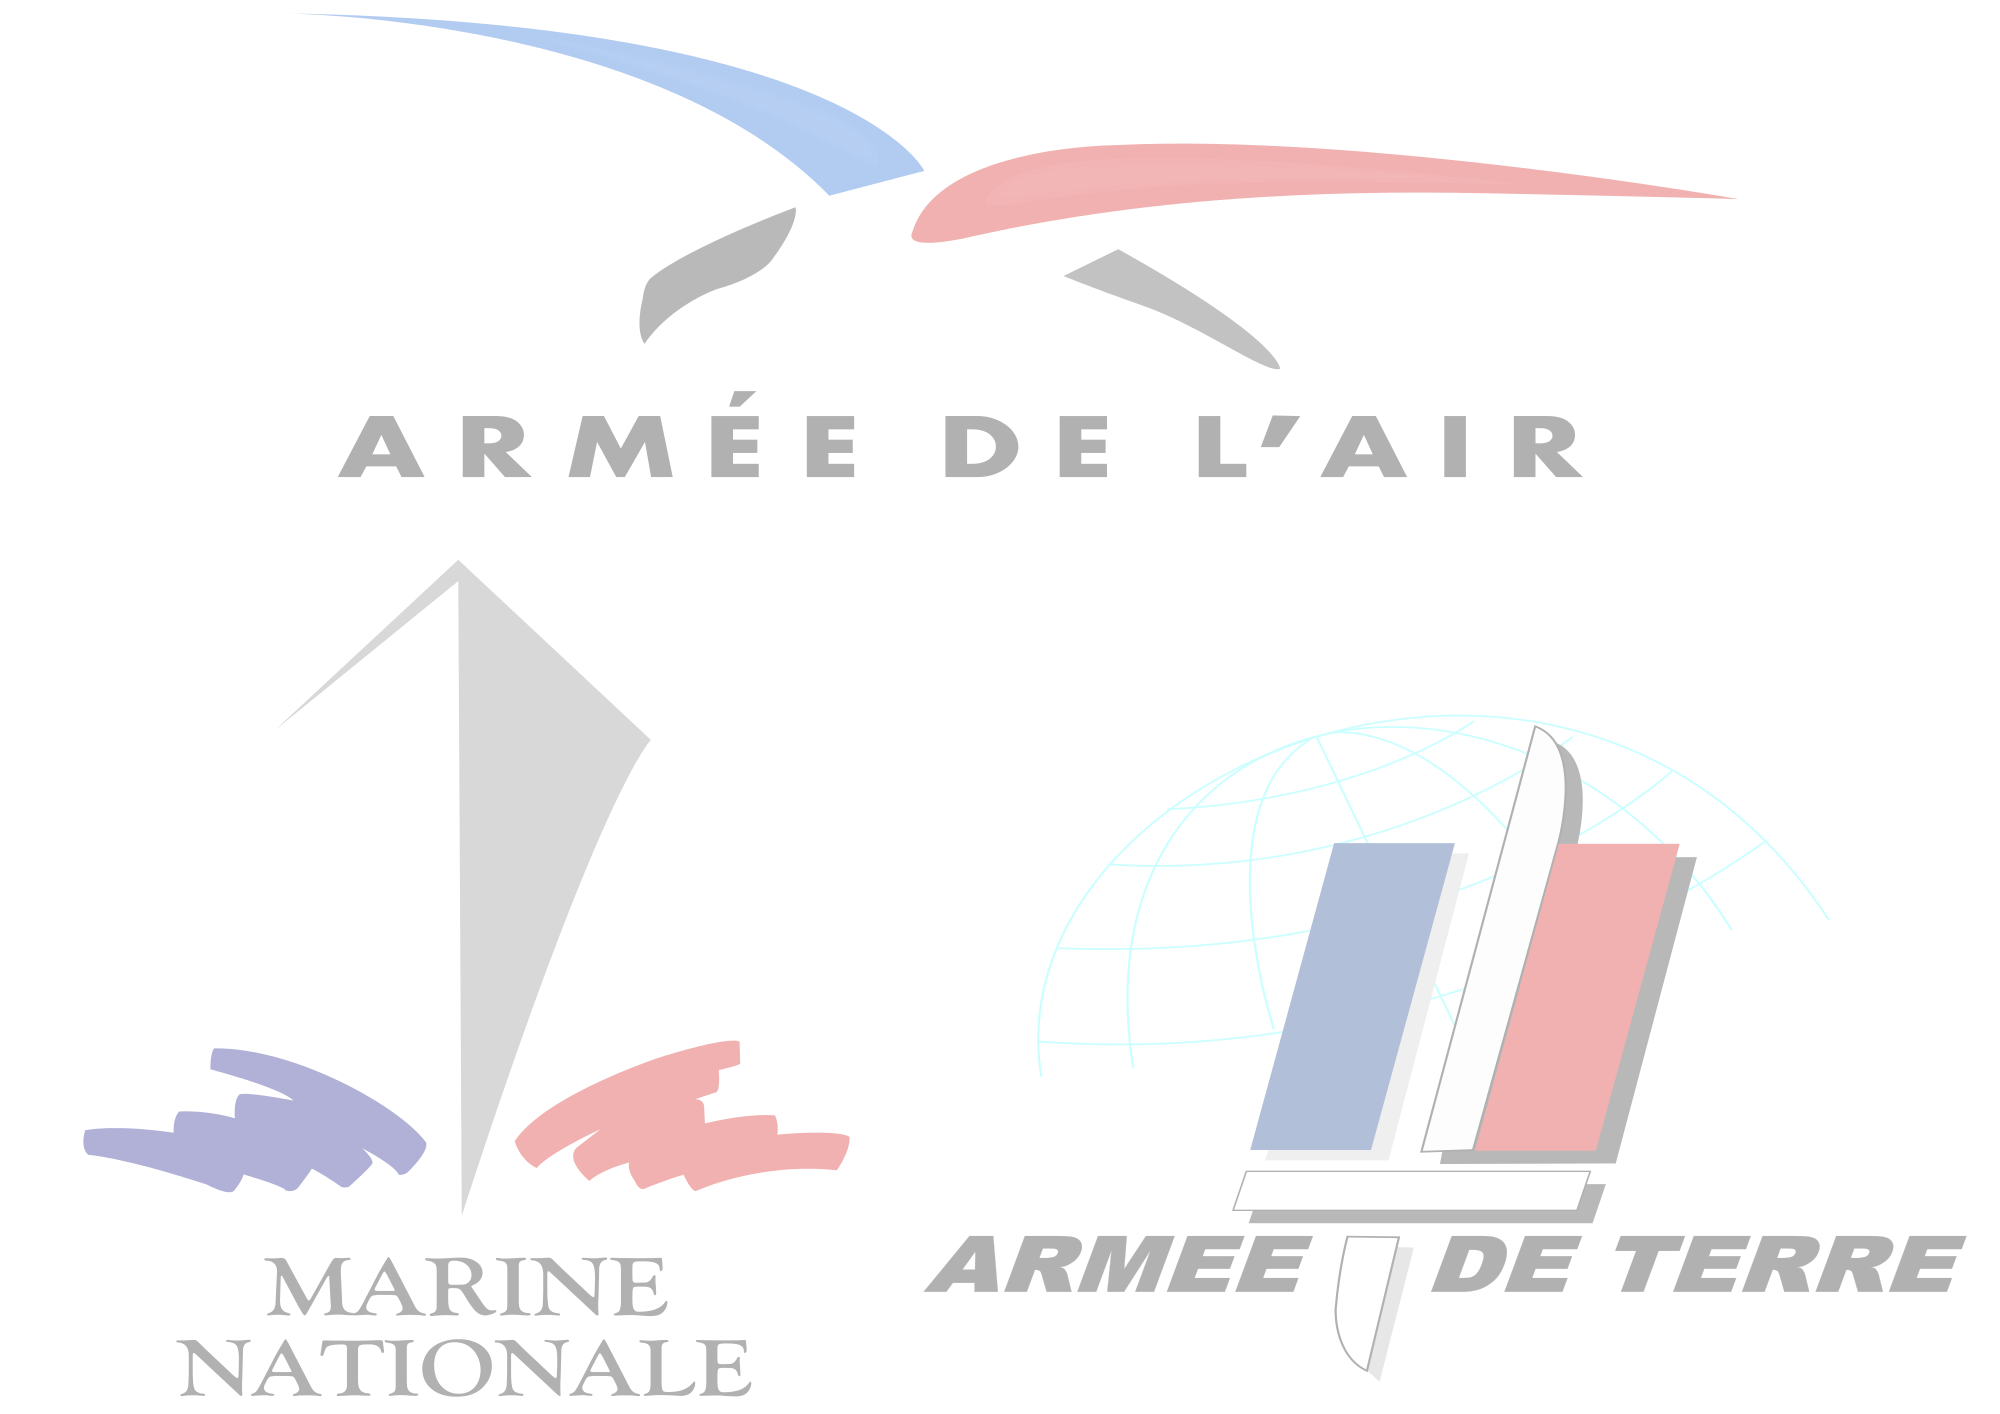
\includegraphics[scale=0.1]{Logo_of_the_French_Armed_Forces}}}
\begin{frame}{Quelques employeurs}{Les Armées}

    \begin{itemize}
        \item Nombreux niveaux d'entrées
        \item Bonne évolution professionnelle
        \item Expérience reconnue par le privé
        \item Nécessite d'être sportif
        \item Tout militaire quelque soit son poste doit être prêt à donner sa vie pour son pays
    \end{itemize}
    
\end{frame}
}

{ 
\usebackgroundtemplate{\parbox[c][\paperheight][c]{\paperwidth}{\centering
\includegraphics[scale=0.4]{DGSE_logo}}}
\begin{frame}{Quelques employeurs}{La DGSE}

    \begin{itemize}
        \item Entrée très restreinte
        \item Accepte autant des civils que des militaires
        \item Chargé du renseignement provenant de l'étranger
        \item Serait responsable des actions menées par la France sur des réseaux étrangers
    \end{itemize}
    
\end{frame}
}

{ 
\usebackgroundtemplate{\parbox[c][\paperheight][c]{\paperwidth}{\centering
\includegraphics[scale=0.4]{logo_dgsi}}}
\begin{frame}{Quelques employeurs}{La DGSI}

    \begin{itemize}
        \item Entrée très restreinte
        \item Service uniquement composé par des civils
        \item Originellement ses ancêtres étaient rattachés à la Police Nationale
        \item Chargé du renseignement provenant de l'intérieur et des éventuelles surveillances sur le territoire national
    \end{itemize}
    
\end{frame}
}

{ 
\usebackgroundtemplate{\parbox[c][\paperheight][c]{\paperwidth}{\centering
\includegraphics[scale=0.1]{Anssi}}}
\begin{frame}{Quelques employeurs}{L'ANSSI}

    \begin{itemize}
        \item Service très spécialisé chargé d'assurer la protection des SI publics comme privés français en réalisant des audits et des sensibilisation par exemple
        \item Service relativement jeune mais qui semble très ouvert
        \item Plusieurs offres d'emplois et de stages
        
    \end{itemize}
    
\end{frame}
}

\begin{frame}{Quelques employeurs}{Les Universités}

Le parcours parfait pour la recherche dans le Public, parcours que je ne détaillerai pas puisque vous avez déjà les pieds dedans.

\end{frame}

\subsection{Secteur Privé}

\begin{frame}{Exemples de métiers}
    
    \begin{itemize}
        \item Informatique \begin{itemize}
            \item Auditeur
            \item \emph{Pen-tester}
            \item Expert en Sécurité des Systèmes d'Information
            \item \dots
        \end{itemize}
        \item Physique \begin{itemize}
            \item Expert en Télécommunication
            \item \dots
        \end{itemize}
    \end{itemize}
    
\end{frame}

\begin{frame}{Quelques employeurs}{Les SSII}

De très nombreux postes liés à l'informatique sont offerts dans les SSII puisqu'il s'agit de leur domaine d'action. Mais avec le nombre croissant d'attaques informatiques de plus en plus de postes ont attrait à la cyberprotection. Que ce soit dans la mise en place d'une (meilleure) sécurité de système d'information ou dans le conseil les SSII restent les maîtres incontestés des services liés au numérique.
    
\end{frame}

\begin{frame}{Quelques employeurs}{Les entreprises d'intérêt stratégiques}

La cyberguerre est pour certaines entreprises un cauchemar duquel elle ne se réveilleront jamais. En effet pour les entreprises comme Dassault Aviation, DCNS, Total et tant d'autres elles représentent le summum des capacités stratégiques et technologiques de la France et sont donc des cibles de choix pour les différents acteurs de la guerre numérique. Ainsi elles doivent redoubler d'efforts pour se protéger des attaques et intrusions. Et ainsi elle sont particulièrement à la recherche de personnels qualifiés dans les domaines de la cyberprotection. Le seul défaut est qu'elles recherchent des personnes ayant déjà une grande expérience.
    
\end{frame}

\section{Conclusion}

\begin{frame}{Pour conclure}
  
  \begin{itemize}
  \pause \item Quoi qu'on en dise, quel que soit le nom qu'on lui donne \alert{la cyberguerre est une réalité}.
  \pause \item Les acteurs sont \alert{nombreux, plus ou moins dangereux et organisés} et chacun avec leurs agendas spécifiques.
  \pause \item Cependant les gouvernements comme les entreprises s'en rendent compte et \alert{la guerre numérique créée des emplois}.
  \end{itemize}

\end{frame}

\begin{frame}{Remerciements}
    Merci beaucoup d'avoir suivi cette conférence.\\
    Si vous avez des questions je vous invite à les poser maintenant.\\
    
    \uncover<2->{%
    Cette présentation est maintenant terminée, en espérant qu'elle vous ait plu, des cookies devraient vous attendent à la sortie de l'amphithéâtre.
    
    \begin{figure}[h]
        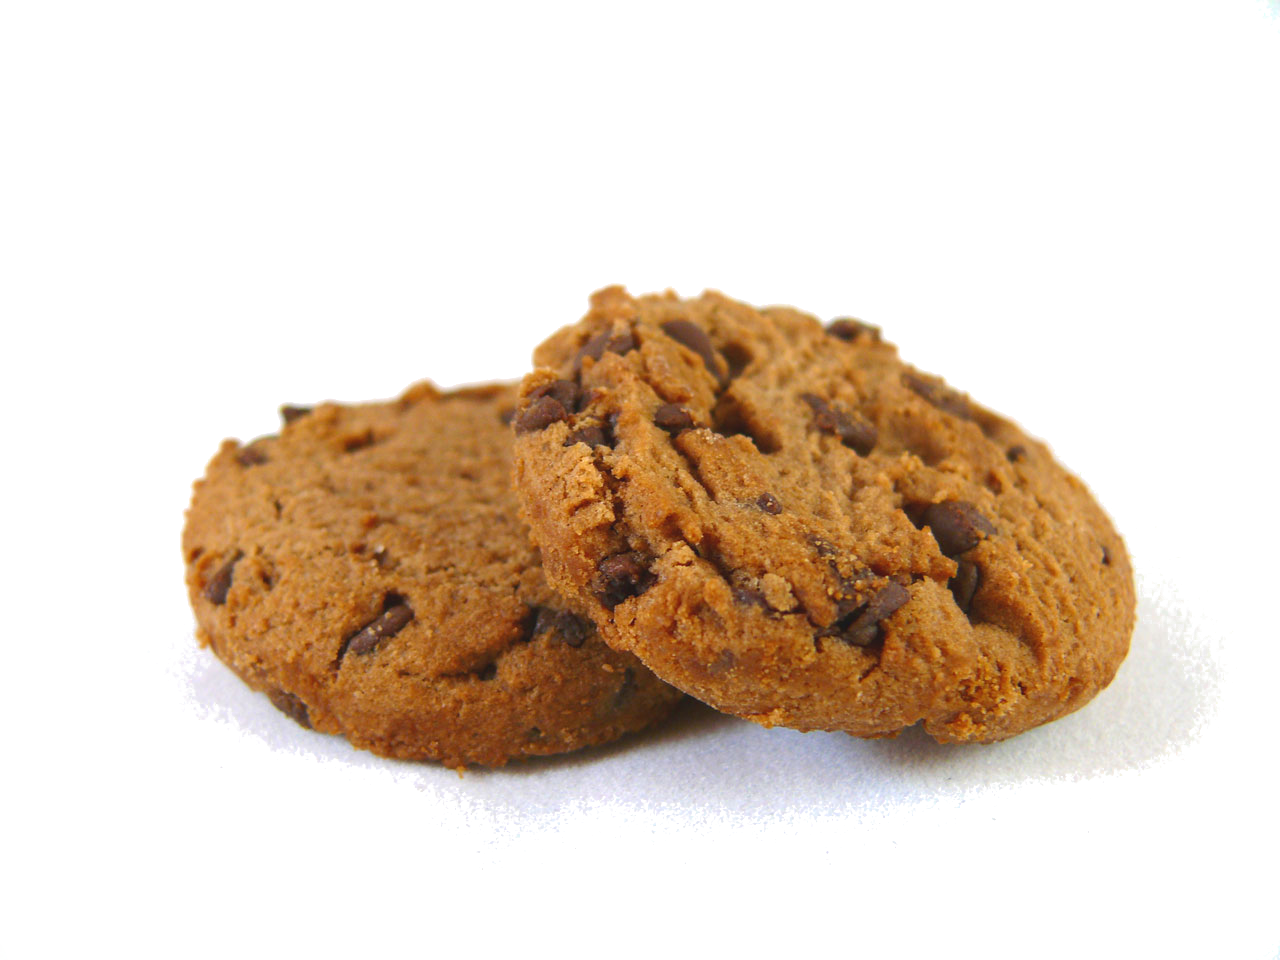
\includegraphics[scale=0.1]{Cookie}
    \end{figure}
    }
    
\end{frame}

\end{document}